\mansection{tril and triu}
\begin{mandesc}
  \short{tril}{extract a lower triangle of the matrix}\\
  \short{triu}{extract an upper triangle of the matrix}
\end{mandesc}
%-- Calling sequence section
\begin{calling_sequence}
\begin{verbatim}
  B = tril(A)
  B = tril(A,k)
  
  B = triu(A)
  B = triu(A,k)
\end{verbatim}
\end{calling_sequence}
%-- Parameters
\begin{parameters}
  \begin{varlist}
    \vname{A}: matrix (full or sparse).
    \vname{k}: optional argument, must be an integer (default is $0$)
    \vname{B}: matrix (full or sparse).
  \end{varlist}
\end{parameters}
\begin{mandescription}
  \verb+tril(A,k)+ extracts the lower triangle of the matrix $A$ ``until'' the diagonal number $k$
  (this one comprised) while the \verb+triu(A,k)+ extracts the upper triangle ``from'' the  diagonal
  number $k$. The matrix element $A_{i,j}$ is located on the diagonal number $j-i$. So main 
  diagonal is numbered $0$, the diagonal number $1$ and $-1$ are respectively located just 
  upper and under the main diagonal, etc...
  $$
  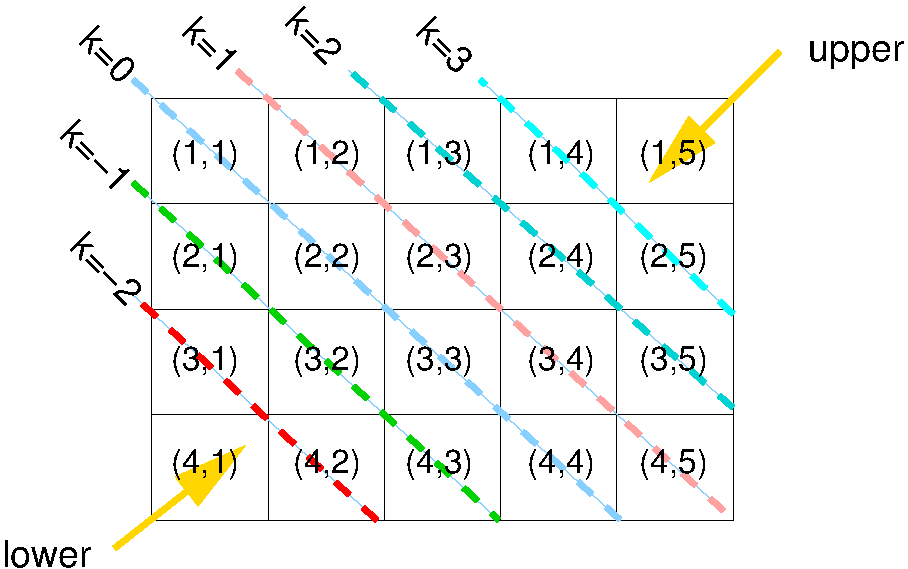
\includegraphics[width=8cm]{\mansrc basicnumarrays/diagonal} 
  $$
  More precisely, if $A$ is a $m \times n$ then   $B = tril(A,k)$ and $C=triu(A,k)$ are both $m \times n$ matrices and:

%%   $$
%%   \begin{array}{l}
%%     B_{i,j} = \left\{ \begin{array}{l} A_{i,j} \mbox{ if } j-i \le k \\
%%       0    \mbox{ otherwise}
%%     \end{array} \right.   \\
%%     C_{i,j} = \left\{ \begin{array}{l} A_{i,j} \mbox{ if } j-i \ge k \\
%%       0    \mbox{ otherwise}
%%     \end{array} \right. 
%%   \end{array}
%%   $$

  \begin{align*}
  B_{i,j} &= 
  \begin{cases}
    A_{i,j} & \text{ if $j-i \le k$}, \\
    0  &  \text{ otherwise.}
  \end{cases} \\
  C_{i,j} &= 
  \begin{cases}  A_{i,j} &\text{ if $j-i \ge k$}, \\
      0   & \text{ otherwise}.
  \end{cases}
  \end{align*}

\end{mandescription}
%--example 
\begin{examples}
\begin{mintednsp}{nsp}
A=rand(4,5) 
tril(A) 
tril(A,-1) 
tril(A,1) 
triu(A) 
triu(A,-1) 
triu(A,1)
\end{mintednsp}
\end{examples}

%-- see also
\begin{manseealso}
  \manlink{diag}{diag}
\end{manseealso}

